The system to be developed is inserted in a network, more specifically, an infrastructure based network, as shown in figure \ref{fig:infr_based_arch}. This type of networks are composed by wireless segments of a more extensive network, whose core is usually a wired network. Infrastructure-based networks have a special station, called an \ac{ap} or  \ac{bs}, which serves as an interface between the wireless segment and the rest of the network. Inside the wireless segment, there will be a centralized communication, so that all messages that circulate on the network pass through a central station. That way, the network only supports two transmission directions: the downward direction (downlink), from the central station to the central station, and the uplink direction, from the stations to the central station. The downlink usually allows the simultaneous transmission of information to a group of stations in the cell (multicast) or to all stations (broadcast).

\begin{figure}[ht]
	\centering
	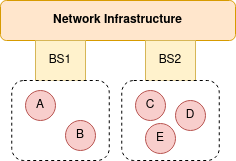
\includegraphics[width=.36\textwidth]{/03system_overview/infrastructure_based}
	\caption{Infrastructure based network architecture.}
	\label{fig:infr_based_arch}
\end{figure}

Street lighting is generally divided into sectors, facilitating maintenance and problem solving regarding the lighting network. So, the system to be developed is a Base Station, in a network of other systems that also contribute to the smart management of that lighting network. This base station is a “special station”, since it connects the local network of lighting poles to other base stations, and also because it has a camera for the detection of available parking spaces. The rest of the stations, that compose the local network, will only do the smart management of their lamps.

\begin{figure}[ht]
	\centering
	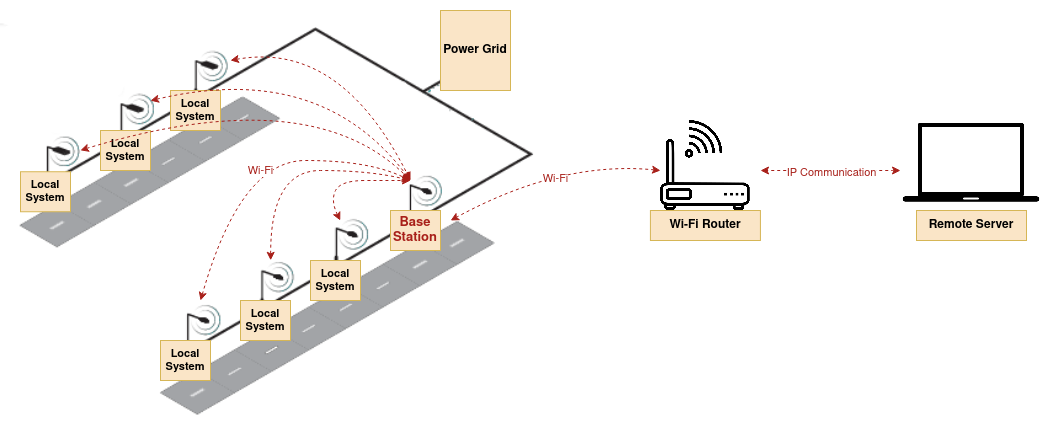
\includegraphics[width=1\textwidth]{/03system_overview/network_arch}
	\caption{Network architecture.}
	\label{fig:network_arch}
\end{figure}